\documentclass[conference,final,]{IEEEtran}


\usepackage{graphicx}
\makeatletter
\def\maxwidth{\ifdim\Gin@nat@width>\linewidth\linewidth
\else\Gin@nat@width\fi}
\makeatother
\let\Oldincludegraphics\includegraphics
\renewcommand{\includegraphics}[1]{\Oldincludegraphics[width=\maxwidth]{#1}}

\usepackage[unicode=true]{hyperref}
\usepackage[spanish]{babel}
\usepackage[utf8]{inputenc} 
\usepackage[T1]{fontenc}
\usepackage{lmodern}
\usepackage{natbib}
\bibliographystyle{apalike}

\hypersetup{
            pdftitle={Análisis de variables climáticas del páramo la Rusia perteneciente al departamento de Boyacá},
            pdfkeywords={keyword 1, keyword 2},
            pdfborder={0 0 0},
            breaklinks=true}
\urlstyle{same}  % don't use monospace font for urls

% Pandoc toggle for numbering sections (defaults to be off)
\setcounter{secnumdepth}{0}

% Pandoc syntax highlighting


% Pandoc header

\providecommand{\tightlist}{%
  \setlength{\itemsep}{0pt}\setlength{\parskip}{0pt}}

%% END MY ADDITIONS %%


\hyphenation{op-tical net-works semi-conduc-tor}

\begin{document}
%
% paper title
% Titles are generally capitalized except for words such as a, an, and, as,
% at, but, by, for, in, nor, of, on, or, the, to and up, which are usually
% not capitalized unless they are the first or last word of the title.
% Linebreaks \\ can be used within to get better formatting as desired.
% Do not put math or special symbols in the title.
\title{Análisis de variables climáticas del páramo la Rusia perteneciente al
departamento de Boyacá}

% author names and affiliations
% use a multiple column layout for up to three different
% affiliations

\author{

%% ---- classic IEEETrans wide authors' list ----------------
 % -- end affiliation.wide
%% ----------------------------------------------------------



%% ---- classic IEEETrans one column per institution --------
 %% -- beg if/affiliation.institution-columnar
\IEEEauthorblockN{
  %% -- beg for/affiliation.institution.author
Camilo Andres Cruz Sanchez %% -- end for/affiliation.institution.author
}
\IEEEauthorblockA{Departamento de Ciencias Forestales\\
Universidad Nacional de Colombia\\
Medellín, Antioquia
\\cacruzs@unal.edu.co
}
\and
\IEEEauthorblockN{
  %% -- beg for/affiliation.institution.author
Natali Andrea Lopez Toro %% -- end for/affiliation.institution.author
}
\IEEEauthorblockA{Area Curricular de Medio Ambiente\\
Universidad Nacional de Colombia\\
Medellín, Antioquia
\\naalopezto@unal.edu.co
}
\and
\IEEEauthorblockN{
  %% -- beg for/affiliation.institution.author
Juan David Leon Torres %% -- end for/affiliation.institution.author
}
\IEEEauthorblockA{Departamento de Ciencias Forestales\\
Universidad Nacional de Colombia\\
Medellín, Antioquia
\\judleonto@unal.edu.co
}
\and
\IEEEauthorblockN{
  %% -- beg for/affiliation.institution.author
Cristian Camilo Gañan Tapasco %% -- end for/affiliation.institution.author
}
\IEEEauthorblockA{Departamento de Ciencias Forestales\\
Universidad Nacional de Colombia\\
Medellín, Antioquia
\\ccganant@unal.edu.co
}
 %% -- end for/affiliation.institution
 %% -- end if/affiliation.institution-columnar
%% ----------------------------------------------------------





%% ---- one column per author, classic/default IEEETrans ----
 %% -- end if/affiliation.institution-columnar
%% ----------------------------------------------------------

}

% conference papers do not typically use \thanks and this command
% is locked out in conference mode. If really needed, such as for
% the acknowledgment of grants, issue a \IEEEoverridecommandlockouts
% after \documentclass

% for over three affiliations, or if they all won't fit within the width
% of the page, use this alternative format:
%
%\author{\IEEEauthorblockN{Michael Shell\IEEEauthorrefmark{1},
%Homer Simpson\IEEEauthorrefmark{2},
%James Kirk\IEEEauthorrefmark{3},
%Montgomery Scott\IEEEauthorrefmark{3} and
%Eldon Tyrell\IEEEauthorrefmark{4}}
%\IEEEauthorblockA{\IEEEauthorrefmark{1}School of Electrical and Computer Engineering\\
%Georgia Institute of Technology,
%Atlanta, Georgia 30332--0250\\ Email: see http://www.michaelshell.org/contact.html}
%\IEEEauthorblockA{\IEEEauthorrefmark{2}Twentieth Century Fox, Springfield, USA\\
%Email: homer@thesimpsons.com}
%\IEEEauthorblockA{\IEEEauthorrefmark{3}Starfleet Academy, San Francisco, California 96678-2391\\
%Telephone: (800) 555--1212, Fax: (888) 555--1212}
%\IEEEauthorblockA{\IEEEauthorrefmark{4}Tyrell Inc., 123 Replicant Street, Los Angeles, California 90210--4321}}




% use for special paper notices
%\IEEEspecialpapernotice{(Invited Paper)}




% make the title area
\maketitle

% As a general rule, do not put math, special symbols or citations
% in the abstract
\begin{abstract}
Los páramos son ecosistemas muy complejos e importantes por el papel que
juegan en la regulación y conservación del recurso hídrico, estos
ecosistemas de alta montaña son el lugar donde nacen múltiples canales
que alimentan a los grandes ríos, nuestro país es rico en estos
ecosistemas pues casi la mitad de todos los páramos se encuentran en
nuestro país, específicamente sobre las tres cordilleras andinas. En el
departamento de Boyacá se encuentra el páramo La Rusia que es el lugar
de donde se han tomado los datos climáticos para este artículo. En este
se analizan los datos de precipitación, temperatura, humedad relativa,
radiación solar, velocidad y dirección del viento tomados de una
estación climática de este páramo y registrados durante un periodo de 6
meses cada 15 minutos, además también se estudian los datos en tiempo
real de de Humedad relativa y temperatura tomados de dos sensores HOBO
en periodos de un minuto, los cuales se registraron durante
aproximadamente los 4 días en que se llevó a cabo la práctica de
campo.\\
Los páramos son ecosistemas muy complejos e importantes por el papel que
juegan en la regulación y conservación del recurso hídrico por lo cual
se hace necesario entender el comportamiento de las variables climáticas
que se presenta en ellos y es por esto que se realiza un estudio en el
páramo de La Rusia donde se toman datos de precipitación, humedad
relativa, temperatura, radiación solar, velocidad y dirección del viento
para 6 meses del año 2019 a través de una estación climatológica que
hace parte de un complejo de estaciones climáticas que ha venido
instalando el equipo de trabajo del Dr.~Mark Mulligan de Kings College y
dos sensores HOBO con los cuales se midieron temperatura y humedad
relativa a través del páramo durante cuatro días del mes de abril. Datos
con los cuales se hicieron relaciones entre las diferentes variables
climáticas por medio del software R los cuales mostraron correlaciones
positivas para la humedad relativa y precipitación(0.38) y correlaciones
negativas entre la radiación y humedad relativa(-0.81). Para los datos
de los sensores se realizó un modelo kriging ordinario de primer orden y
transformación logarítmica por medio del software Arcgis, el cual mostró
una disminución en la temperatura a medida que se aumentaba la altitud,
pero no con una relación lineal sino que era fluctuante.
\end{abstract}

% keywords
\begin{IEEEkeywords}
keyword 1; keyword 2
\end{IEEEkeywords}

% use for special paper notices



% make the title area
\maketitle

% no keywords

% For peer review papers, you can put extra information on the cover
% page as needed:
% \ifCLASSOPTIONpeerreview
% \begin{center} \bfseries EDICS Category: 3-BBND \end{center}
% \fi
%
% For peerreview papers, this IEEEtran command inserts a page break and
% creates the second title. It will be ignored for other modes.
\IEEEpeerreviewmaketitle


\hypertarget{introducciuxf3n}{%
\section{Introducción}\label{introducciuxf3n}}

El páramo es uno de los ecosistemas más importantes para la captura de
agua, este se encuentra presente en un \(99 \%\) en la Cordillera de los
Andes, en la Sierra Nevada de Santa Marta y Costa Rica, pero también
existen Páramos en África, Indonesia y Papua Nueva Guinea
\cite{cabrera}. Es por esto que los páramos ubicados en la Cordillera de
los Andes han sido definidos como extensas zonas en la cima de la
cordilleras, entre el bosque andino y el límite inferior de las nieves
perpetuas \cite{cabrera}, haciendo privilegiados a los pocos países en
el mundo que cuentan con este tipo de ecosistema por la riqueza acuífera
que ellos representan. Para el caso de Colombia en el que se encuentran
el \(49 \%\) de los páramos del mundo, ocupando el \(1.7 \%\) del
territorio nacional con aproximadamente \(34\) páramos \cite{cabrera},de
estos según el ministerio de ambiente, el departamento de Boyacá cuenta
con el \(18.7 \%\) del total nacional. Conteniendo en \(16\) municipios
de este departamento se encuentra el páramo de La Rusia, en el cual se
centrará el presente informe con el fin de conocer y analizar las
variables climáticas que allí se presentan.

La altura a la que se puede encontrar un páramo no es igual para todos
los casos, pues el límite inferior de estos es variable según la
latitud, la vertiente, el clima global y la actividad humana. En América
se encuentran entre los \(3000\) y \(4800 \ msnm\) aproximadamente, para
Colombia, en las cordilleras central y occidental está a \(3500 \ msnm\)
y en la oriental a \(3600 \ msnm\). La zonificación típica utilizada en
la alta montaña colombiana corresponde a bosque alto andino (\(3000\) a
\(3200 \ msnm\)), páramo bajo o subpáramo (entre \(3200\) y \(3500\) o
\(3600 \ msnm\)), páramo propiamente dicho (entre \(3500\) o \(3600\) y
\(4100 \ msnm\)) y superpáramo (entre \(4100\) y \(4500 \ msnm\))
\cite{ortizparamos}. Diferentes autores confirman que el clima en los
páramos realmente es muy variado, aunque se presenten condiciones de
altura similares y proximidad \cite{paramos}, esta variabilidad se
presenta en todas las características climáticas, tales como
precipitación, temperatura, radiación, velocidad del viento y humedad
relativa, y aunque hay todavía pocas estaciones climáticas en todos los
páramos es evidente la variación en los resultados de la medición de
estos parámetros climáticos.

Por lo general en la transición de bosque y el subpáramo las
temperaturas medias multianuales en algunos caso pueden ser incluso
menores a \(9^{\circ}C\), aproximadamente por encima de los
\(3300 \ msnm\), en el páramo medio podrían llegar a ser menores de
\(6^{\circ}C\) y ya en el superpáramo cerca de las nieves perpetuas son
inferiores a \(3^{\circ}C\) \cite{morales2019atlas}. En cuanto a la
variación de la temperatura media mensual no hay grandes cambios, sin
embargo en los páramos la temperatura puede variar a gran escala durante
el día y la noche. En la precipitación hay una amplio rango y un gran
contraste entre los páramos de Colombia, la precipitación puede variar
entre los \(700\) y \(5000 \ mm\) al año, algunos de los páramos tienen
un régimen de lluvias monomodal como el páramo chingaza
\cite{morales2019atlas} y otros bimodal como el complejo Guantiva - La
Rusia \cite{morales2019atlas}; los páramos secos se encuentran en las
vertientes oriental de la cordillera oriental y occidental de la
cordillera occidental, en cuanto a los más secos se encuentran entre la
cordillera oriental \cite{morales2019atlas}. Los ecosistemas de páramo
presenta una humedad relativa alta que es variable y estacional siendo
máxima en tiempos de lluvia y mínima en tiempos secos, usualmente en un
rango que comprende entre un \(80\) y \(90 \%\) esto debido a un factor
de suma importancia en los páramos como lo es el fenómeno de niebla
\cite{morales2019atlas}. Comúnmente la evapotranspiración en los páramos
es baja pues casi siempre el ambiente es muy cercano a la saturación y
se presenta un alta radiación ultravioleta sobre todo en periodos secos
y abundancia de luz difusa \cite{morales2019atlas}. Por último los
vientos en los páramos son muy variables pero regularmente los más
intensos se dan en los páramos que se encuentran en las vertientes de
los valles interandinos \cite{morales2019atlas}.

\hypertarget{materiales-y-muxe9todos}{%
\section{MATERIALES Y MÉTODOS}\label{materiales-y-muxe9todos}}

\hypertarget{localizaciuxf3n-y-descripciuxf3n-del-uxe1rea-de-estudio}{%
\subsection{Localización y descripción del área de
estudio}\label{localizaciuxf3n-y-descripciuxf3n-del-uxe1rea-de-estudio}}

El páramo la Rusia se encuentra ubicado en límites de los departamentos
de Boyacá y Santander, en el flanco occidental de la cordillera
oriental, entre los \(3100\) y \(4280 \ msmn\). Este páramo hace parte
de un extenso corredor de páramos y bosques alto andinos denominado como
Guantiva - La Rusia, complejo que incluye a los páramos de Cruz
Colorada, Guina, Pan de Azúcar, Carnicerías y Guata y que tiene una
extensión en área de \(119.009 \ ha\) (Corpoboyacá y CAS, 2017), en el
cual predomina una topografía abrupta que varía de acuerdo con la
alternancia de las formaciones geológicas presentes. El páramo está
influenciado por la Zona de Convergencia Intertropical (ZCIT) y el
movimiento de las corrientes de vientos locales e inter tropicales, lo
que genera un régimen húmedo. El régimen de lluvias es bimodal, con una
precipitación máxima entre abril, mayo, octubre y noviembre (UPTC, 2015)

El sitio de estudio se encuentra dentro del páramo La Rusia en la vereda
San alejo, municipio de Duitama Boyacá; contiguo por el norte a los
límites con el municipio de Charalá departamento de Santander con
coordenadas \(5^{\circ}57’48.0"N\) \(73^{\circ}05'16.3"W\) y una altitud
mayor a los \(3500\ msnm\).

\hypertarget{levantamiento-de-informaciuxf3n}{%
\subsection{Levantamiento de
información}\label{levantamiento-de-informaciuxf3n}}

Dentro del páramo de La Rusia se instalaron varias estaciones
climatológicas cercadas las cuales midieron temperatura, humedad
relativa, velocidad y dirección del viento, precipitación y radiación
solar. Para este artículo sólo se tuvo en cuenta una estación
climatológica con datos para 6 meses del año 2019, de enero a junio,
tomados cada 15 minutos para todas las variables mencionadas. La
estación climática de la cual se obtuvieron los datos hace parte de un
complejo de estaciones climáticas que ha venido instalando el equipo de
trabajo del Dr.~Mark Mulligan de Kings College, como parte de un
proyecto para probar y calibrar equipos de monitoreo open source más
rentables para los proyectos investigativos.

También se usaron dos sensores HOBO móviles para recolectar información
de temperatura y humedad relativa en tiempo real con intervalos de 1
minuto, los cuales fueron puestos en funcionamiento a partir del día
jueves 12 de marzo hasta el sábado 14 de marzo de las 8am a las 5pm y
para el día domingo entre las 8am y las 3pm, llevando los sensores por
parte del complejo de páramos Guantiva- La Rusia a la vez que se iban
instalando las estaciones climáticas y se tomaban otros datos como
caudal y muestras de suelos con el resto del grupo de trabajo, datos que
no se tendrán en cuenta en este informe. Así mismo el uso del software
de la misma empresa (HOBO) para dispositivos celulares en el cual se
podían verificar los datos en tiempo real.

\hypertarget{procesamiento-de-los-datos-recolectados}{%
\subsection{Procesamiento de los datos
recolectados}\label{procesamiento-de-los-datos-recolectados}}

Los datos climáticos pueden proporcionar una gran cantidad de
información sobre el medio ambiente atmosférico que afecta a casi todos
los aspectos del esfuerzo humano \cite{Bala}, es por ello que es
importante el análisis estos, para determinar tendencias en las
variables que se puedan interpretar buscando entender el comportamiento
y así tomar decisiones que más convengan. Buscando el filtrado y
análisis de los datos se utilizó \texttt{R\ versión\ 3.6.1} \cite{Rs}. Para los
datos de precipitación se usó la suma de los los valores diarios por mes
y para los demás (temperatura, humedad relativa y velocidad del viento)
los valores promedio. Se graficaron las variables por separado buscando
propensiones para la descripción de cada una de ellas, luego se buscaron
relaciones estadísticas entre variables con el fin de determinar acaso
alguna dependencia entre los datos. Con los datos de temperatura del
sensor HOBO se realizó un modelo kriging ordinario de primer orden y
transformación logarítmica en el software Arcgis versión 10.5 esto con
el fin de observar un comportamiento aproximado de la variable.

\hypertarget{resultados-y-discusiuxf3n}{%
\section{Resultados y discusión}\label{resultados-y-discusiuxf3n}}

En la \textbf{Fig.1} se puede observar la precipitación mensual
discriminada por la cantidad de precipitación de cada día (representados
en colores), en esta escala no se percibe todo el ciclo anual pero si la
temporada de lluvias entre marzo y mayo y parte de una temporada seca a
la que se debe la baja precipitación en febrero, lo que responde al
régimen bimodal del páramo La Rusia. La precipitación total de estos 6
meses suma \(1096.2mm\), una precipitación alta, característica de las
laderas orientadas al occidente, pues las laderas internas de los Andes
están altamente influenciadas por efectos de sombra de lluvia, para las
lluvias que llegan tanto desde la cuenca del Amazonas como de la costa
del Pacífico \cite{buytaert2006hidrologia}.

\begin{figure}
\centering
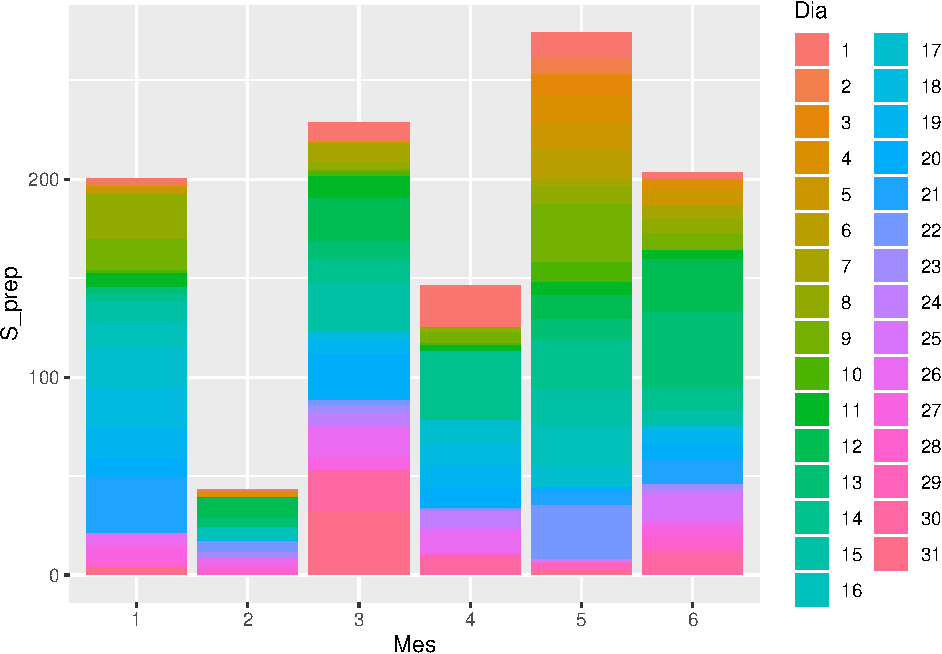
\includegraphics{Hidrology_files/figure-latex/unnamed-chunk-1-1.pdf}
\caption{Tendencia Diaría de precipitación}
\end{figure}

En la \textbf{Fig.2}, se observa la variación de la temperatura
alrededor del promedio de los seis meses de \(9.2^{\circ}C\) con una
temperatura máxima de \(19.5^{\circ}C\) y una mínima de
\(1.6^{\circ}C\), sin embargo la fluctuación de mayor densidad se
encuentra entre los \(8^{\circ}C\) y \(10^{\circ}C\). La variación
diurna de la temperatura resulta del ciclo de insolación superficial
\cite{poveda2004hidroclimatologia}, la cual es mayor entre las 11:00
a.m. y la 1:00 p.m. Debido a su localización cercana a la línea
ecuatorial, la radiación solar diaria es casi constante todo el año.
Esta constancia resulta en una baja variabilidad estacional en
temperatura media del aire, en contraste con el ciclo diario, el cual es
totalmente marcado \cite{buytaert2006hidrologia}.

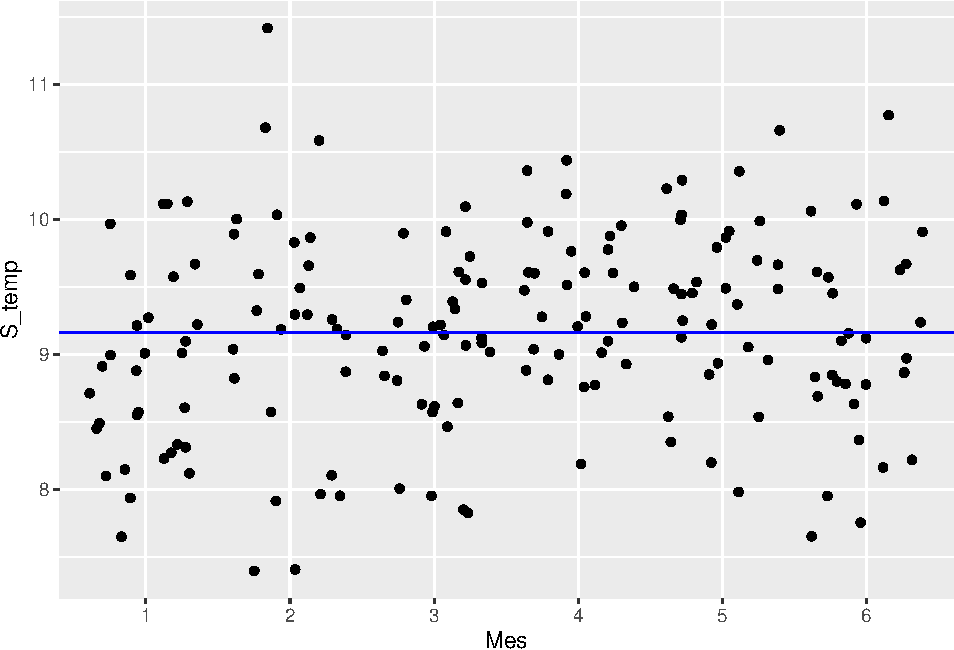
\includegraphics{Hidrology_files/figure-latex/unnamed-chunk-4-1.pdf}
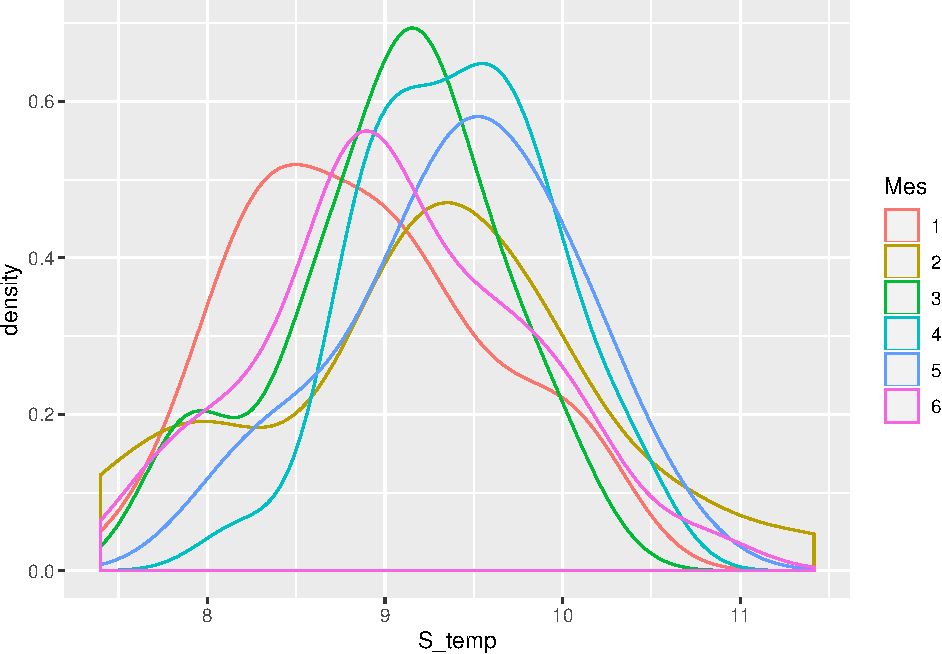
\includegraphics{Hidrology_files/figure-latex/unnamed-chunk-4-2.pdf}

\begin{figure}
\centering
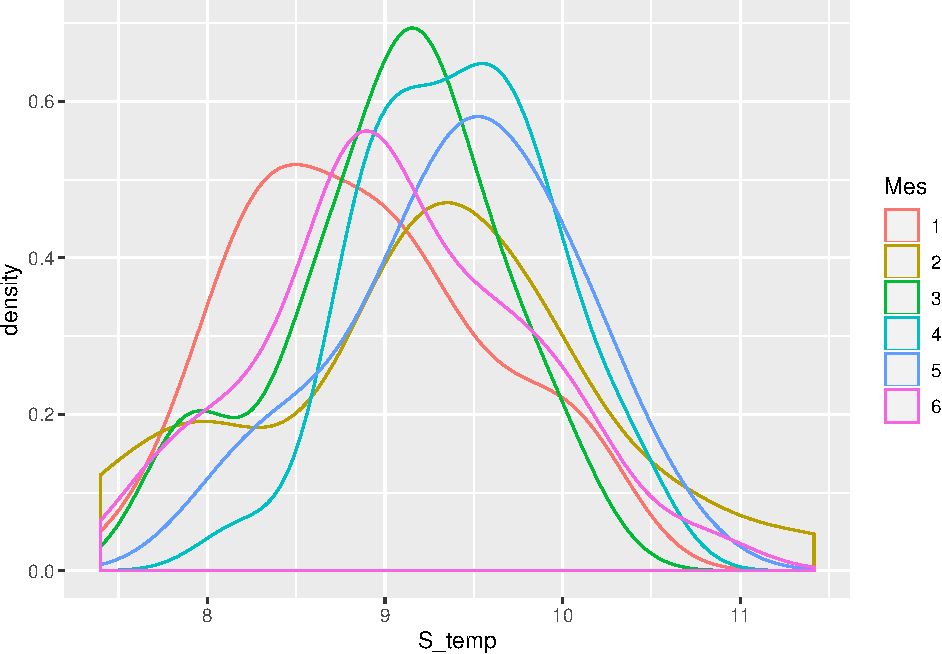
\includegraphics{Hidrology_files/figure-latex/unnamed-chunk-5-1.pdf}
\caption{Temperatura media general}
\end{figure}

\begin{figure}
\centering
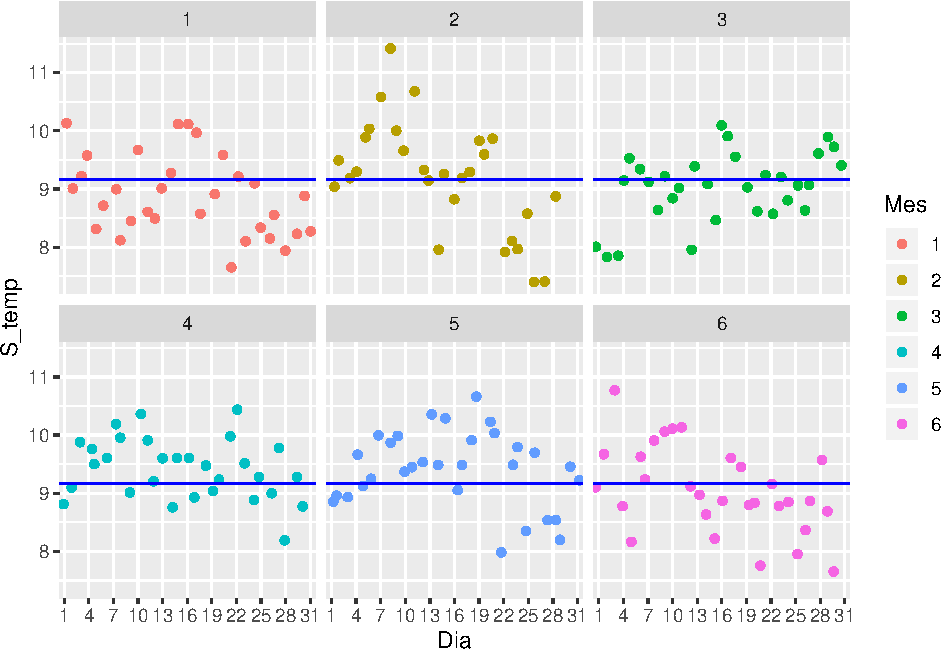
\includegraphics{Hidrology_files/figure-latex/unnamed-chunk-6-1.pdf}
\caption{Analisis de Humedad relativa}
\end{figure}

\begin{figure}
\centering
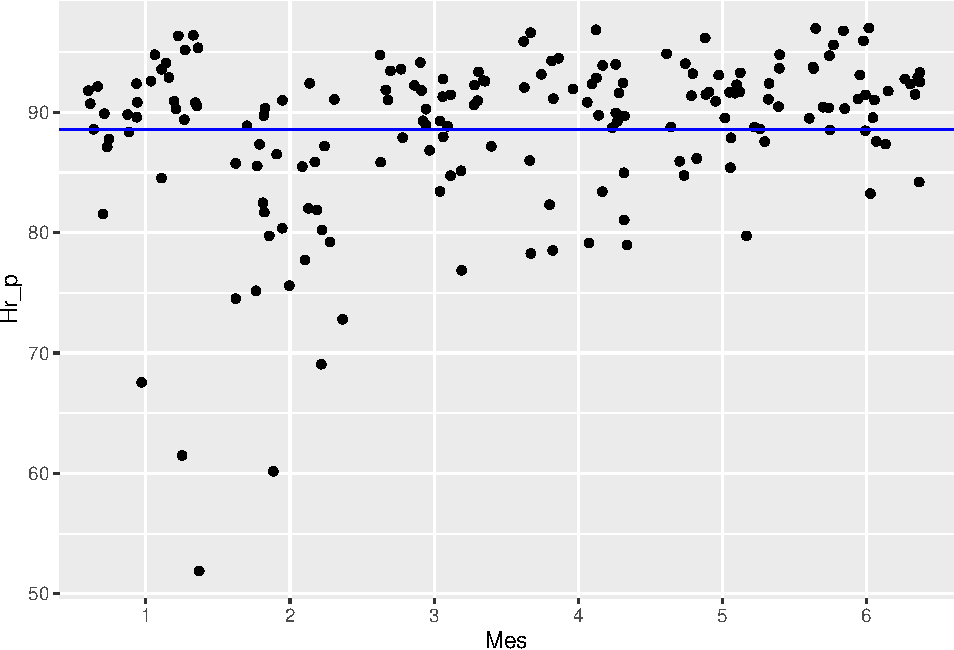
\includegraphics{Hidrology_files/figure-latex/unnamed-chunk-7-1.pdf}
\caption{Analisis de Humedad relativa}
\end{figure}

\begin{figure}
\centering
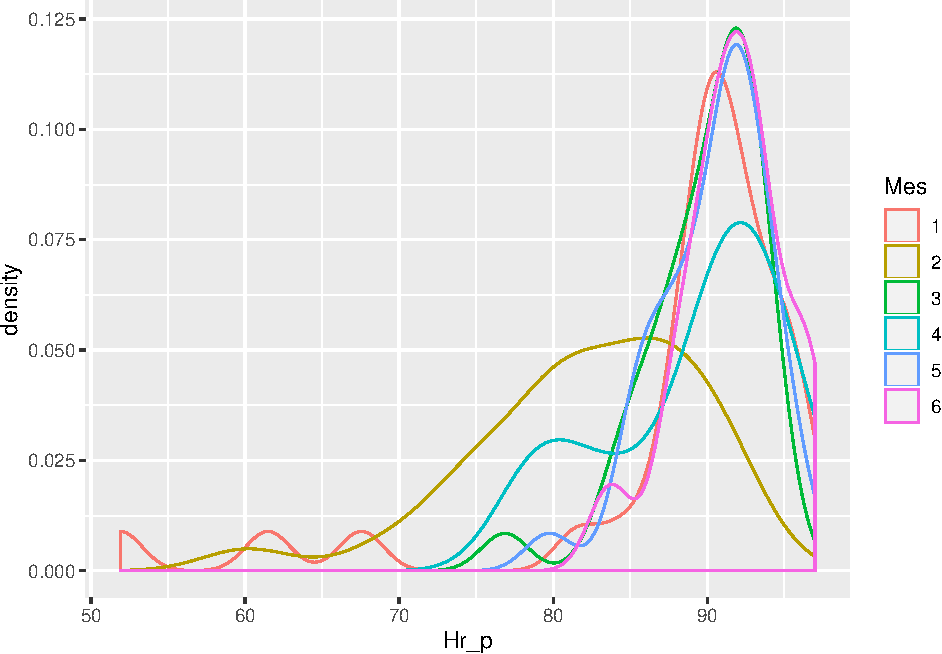
\includegraphics{Hidrology_files/figure-latex/unnamed-chunk-8-1.pdf}
\caption{Analisis de Humedad relativa}
\end{figure}

\begin{figure}
\centering
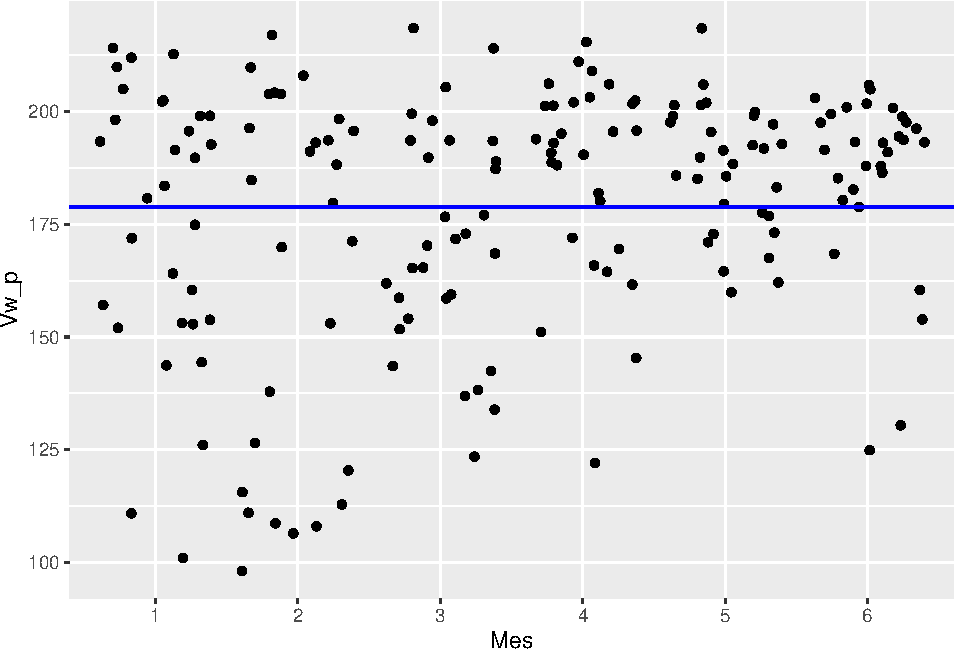
\includegraphics{Hidrology_files/figure-latex/unnamed-chunk-9-1.pdf}
\caption{Analisis de velocidad del viento}
\end{figure}

\begin{figure}
\centering
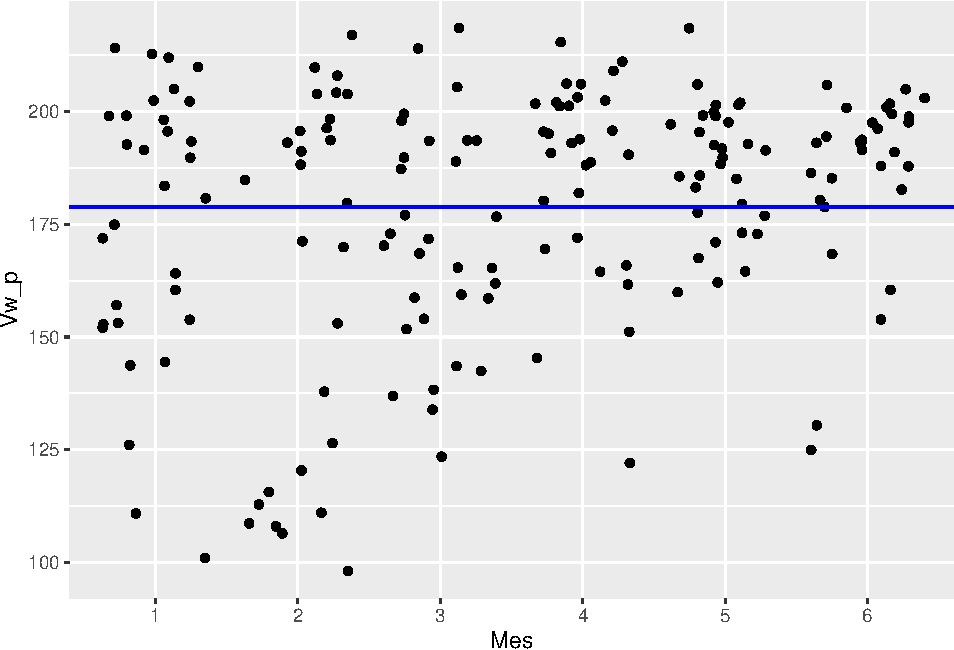
\includegraphics{Hidrology_files/figure-latex/unnamed-chunk-10-1.pdf}
\caption{Analisis de velocidad del viento}
\end{figure}

\begin{figure}
\centering
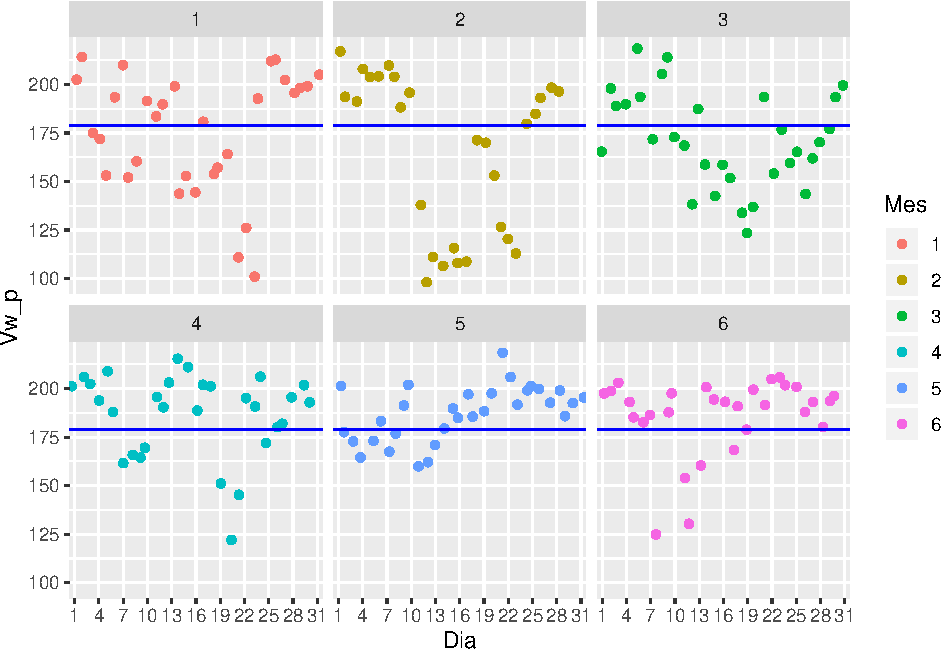
\includegraphics{Hidrology_files/figure-latex/unnamed-chunk-11-1.pdf}
\caption{Analisis de velocidad del viento}
\end{figure}

\begin{figure}
\centering
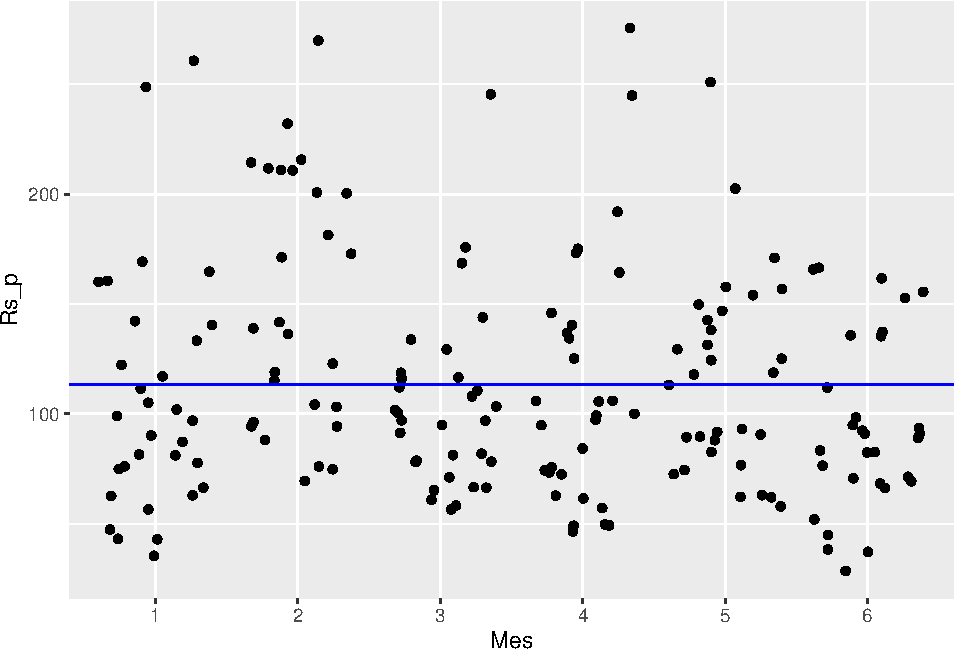
\includegraphics{Hidrology_files/figure-latex/unnamed-chunk-12-1.pdf}
\caption{Radiación solar media}
\end{figure}

\begin{figure}
\centering
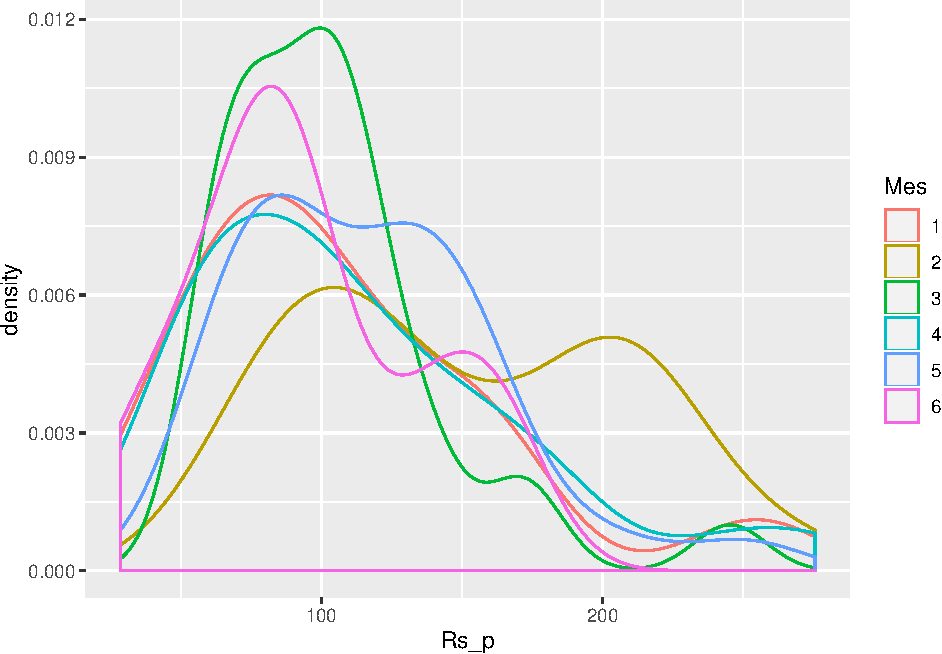
\includegraphics{Hidrology_files/figure-latex/unnamed-chunk-13-1.pdf}
\caption{Radiación solar media}
\end{figure}

\begin{figure}
\centering
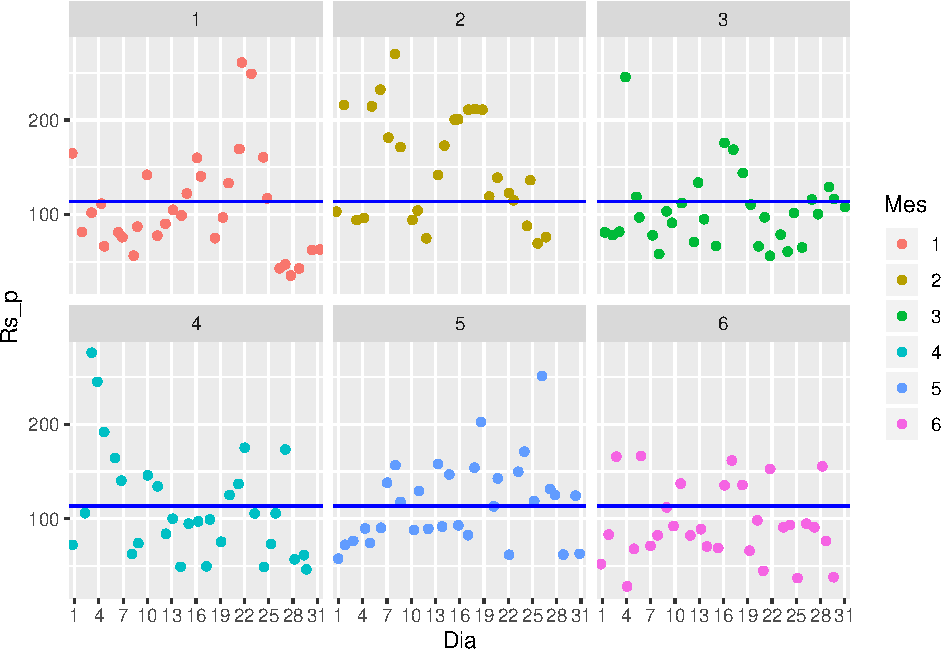
\includegraphics{Hidrology_files/figure-latex/unnamed-chunk-14-1.pdf}
\caption{Radiación solar media}
\end{figure}

En la \textbf{Fig.12} se puede observar la correlación para las
distintas variables climáticas, presentando así una correlación positiva
entre la precipitación y humedad relativa (\(0.38\)), esto puede darse
ya que en épocas de lluvia la humedad relativa es constantemente alta y
tiende a la saturación en eventos de precipitación y además suele
presentarse el fenómeno de niebla. \cite{morales2019atlas}, dato que se
puede corroborar en la \textbf{Fig.15} que muestra la relación entre
precipitación y humedad relativa, que presenta una línea de tendencia
con un aumento muy rápido en la humedad relativa mientras inicia la
precipitación y luego se mantiene constante en el evento de lluvia
tendiendo a la saturación del ambiente. Lo mismo ocurre con las
variables de radiación solar y temperatura que tienen una correlación
positiva de \(0.52\), la cual puede darse por el gran aumento de
insolación solar y temperatura que se presenta a medio día en el páramo
ya que se encuentra muy cerca de la línea ecuatorial y recibe una gran
radiación diaria todo el año mientras se tenga un cielo despejado
\cite{buytaert2006hidrologia}. Esto se puede ver en la \textbf{Fig.14}
que muestra la relación entre temperatura y radiación solar, donde la
línea de tendencia muestra una relación directa en el aumento de la
radiación y temperatura. Caso contrario cuando se analiza la correlación
entre radiación solar y humedad relativa (\(-0.81\)) o temperatura y
humedad relativa (\(-0.25\)), obteniendo valores negativos; esto se pudo
evidenciar en campo, pues mientras la temperatura era más alta el aire
se sentía mucho más seco. Como se puede ver en la \textbf{Fig.13} que
muestra la relación entre temperatura vs humedad relativa, donde la
línea de tendencia disminuye a medida que la temperatura aumenta.

\begin{figure}
\centering
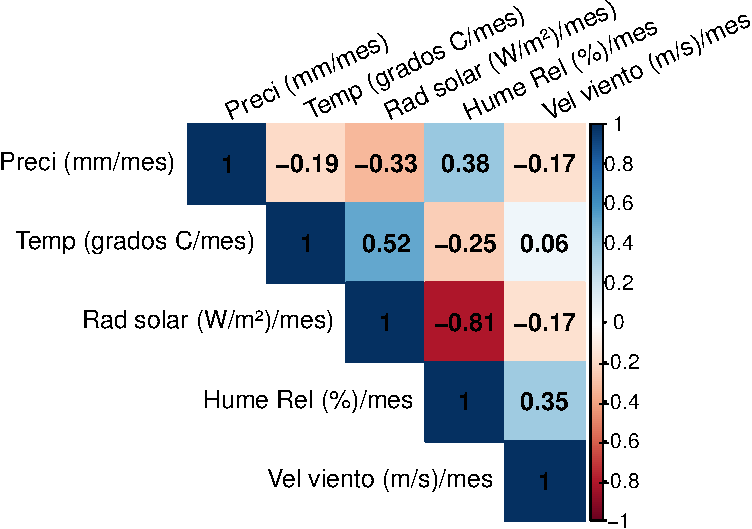
\includegraphics{Hidrology_files/figure-latex/unnamed-chunk-17-1.pdf}
\caption{Matrix de correlación para las variables climáticas}
\end{figure}

\begin{figure}
\centering
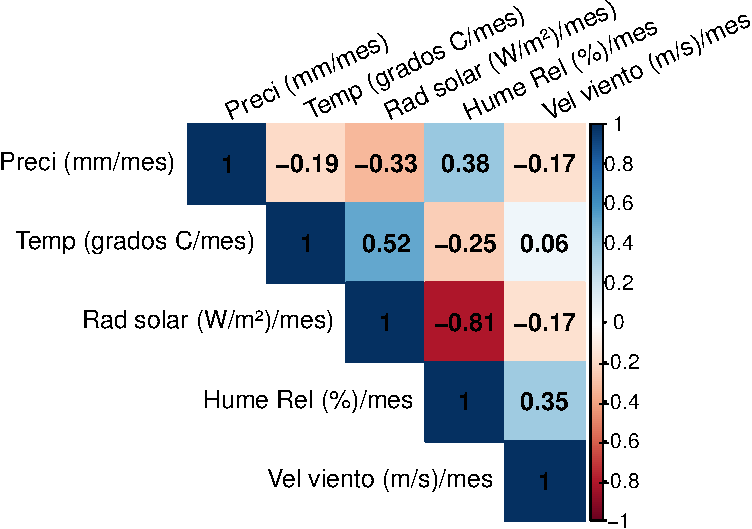
\includegraphics{Hidrology_files/figure-latex/unnamed-chunk-18-1.pdf}
\caption{Temperatura vs Humedad relativa}
\end{figure}

\begin{figure}
\centering
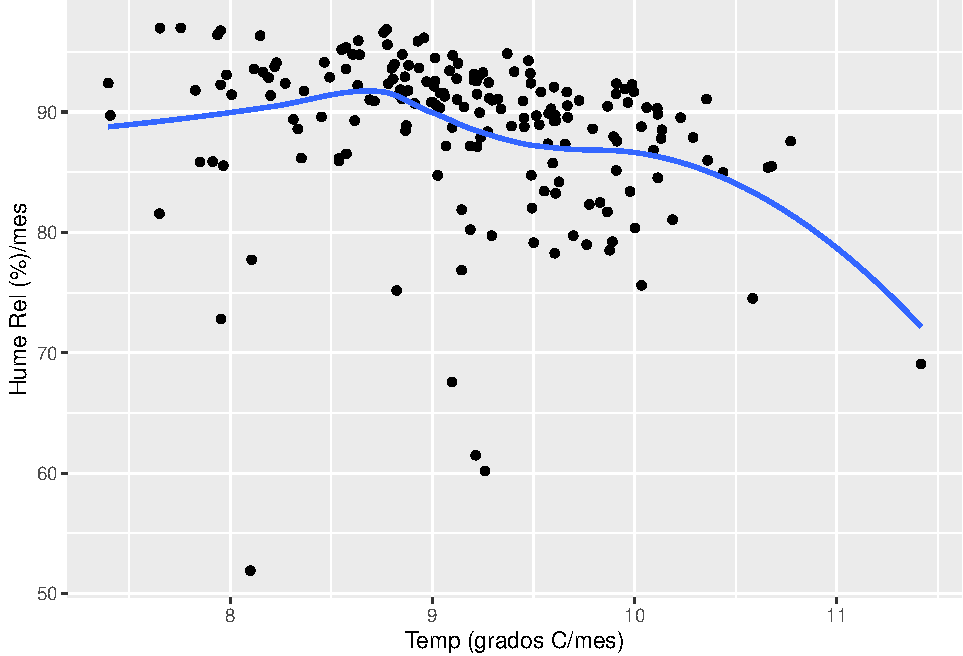
\includegraphics{Hidrology_files/figure-latex/unnamed-chunk-19-1.pdf}
\caption{Temperatura vs Radiación solar}
\end{figure}

\begin{figure}
\centering
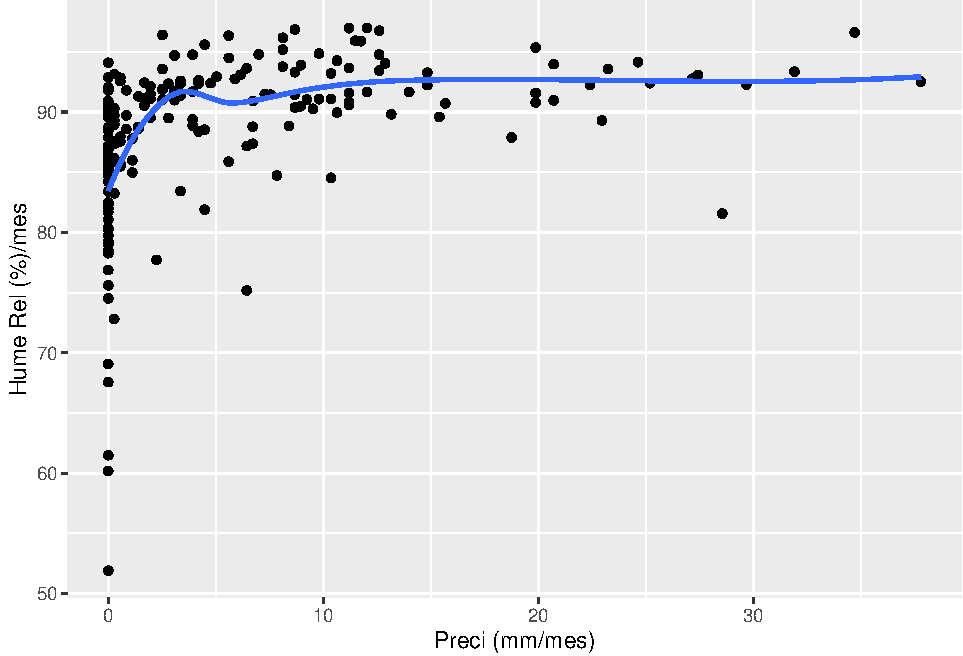
\includegraphics{Hidrology_files/figure-latex/unnamed-chunk-20-1.pdf}
\caption{Precipitación vs Humedad relativa}
\end{figure}

\begin{figure}
\centering
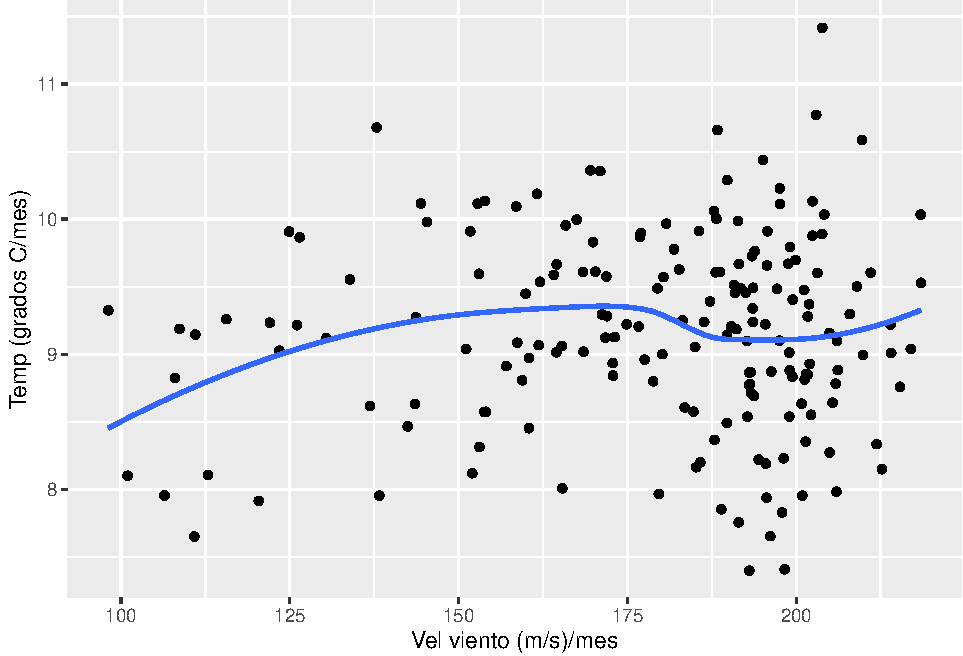
\includegraphics{Hidrology_files/figure-latex/unnamed-chunk-21-1.pdf}
\caption{Velocidad del viento vs Temperatura}
\end{figure}

En la \textbf{Fig.13} se puede observar la reacción que se encontró para
los parámetros climáticos temperatura y humedad relativa durante el
periodo del que se tienen los datos. La gráfica de dispersión ilustra un
comportamiento inverso entre las dos variables con una línea de
tendencia que en general es decreciente, a medida que comienza a
ascender la temperatura la humedad relativa comienza a descender lo que
es normal pues a medida que el ambiente se torna más caliente, el
ambiente se torna más seco lo que en un páramo está sujeto a la
estacionalidad, pues la humedad relativa es variable y estacional
\cite{hofstede2017p}, así en épocas de lluvia habrá mayor humedad
relativa que en épocas secas o de verano, la variación de este factor
está estrechamente ligada a los fenómenos de niebla que en un páramo
pueden presentarse con mayor o menor frecuencia dentro de un periodo de
tiempo. En síntesis la gráfica no se sale del comportamiento normal de
estos dos parámetros climatológicos (humedad relativa y temperatura),
debido a que estos son normalmente inversos, cabe destacar que la
humedad relativa extrañamente baja a valores menores de 70 lo que es
característico de estos ecosistemas. \cite{hofstede2017p}

\begin{figure}
\centering
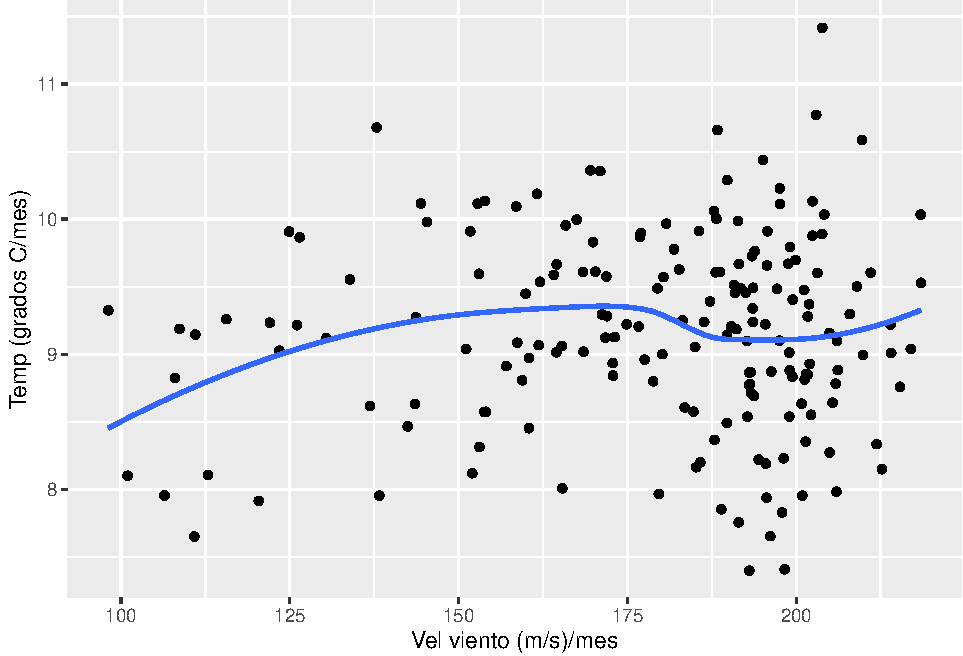
\includegraphics{Hidrology_files/figure-latex/unnamed-chunk-22-1.pdf}
\caption{Distribución empírica acumulada de precipitación}
\end{figure}

En la \textbf{Fig.14} se observa la relación entre la temperatura y la
radiación solar para el páramo La Rusia, de la gráfica se deduce que
estos dos parámetros son generalmente directamente proporcionales pues
en la mayoría del tiempo a medida que la temperatura aumenta la
radiación solar comienza también a aumentar, la radiación solar empieza
a aumentar a mayor medida mientras lo hace también la temperatura y es
que esto mientras se tengan las condiciones necesarias (como un cielo
despejado) es normal en un páramo pues debido a su altitud y cercanía
con el ecuador la radiación solar que reciben estos ecosistemas es alta
mientras no haya nubosidad \cite{montenegro2015estimacion}.

En la \textbf{Fig.18} se muestra el modelo de temperatura construido a
partir de los datos del sensor HOBO, cabe la pena aclarar que este es un
aproximación y no es un modelo que ajuste bien los datos, es válido
decir esto dada la cantidad de puntos utilizados (\(8\)) son pocos pues
se tomaron las coordenadas de los instrumentos instalados. Se puede
notar el gradiente mostrado en el mapa, sugiere la variabilidad de la
temperatura en el páramo; los rangos mostrados difieren en
aproximadamente \(3^{\circ}C\), al mirar este comportamiento, se
procedió a verificar si la altura tenía influencia en la temperatura, lo
esperado sería que este parámetro tuviera influencia \cite{basantes},
para determinar la relación se hace un test de correlación arrojando un
resultado de \(-0.46\) lo cual indica que mientras una variable aumenta
la otra disminuye, sin embargo, el mismo valor en sí es deja en duda es
una relación lineal, pues se encontró un \(R^2\) de \(0.22\), lo que
demuestra que si bien hay relación en entre los parámetros esta puede
fluctuar y no ser constante, es decir, pueden haber lugares altos pero
con temperaturas más altas de lo normal, este comportamiento no sigue
descrito por \cite{van} la tasa de cambio en el promedio de temperatura
con respecto a la altitud, está típicamente entre \(0.6\) y
\(0.7^{\circ}C\) \(100 \ m-1\), esto se explica quizás por que la subida
de temperatura, causada por el efecto invernadero de varios gases
antropogénicos de los cuales el CO2 es el más conocido, es el proceso
fundamental global del cambio climático, esto viene acompañado de otros
efectos secundarios \cite{buyta} los cuales no serán tratados acá.

\begin{figure}
\centering
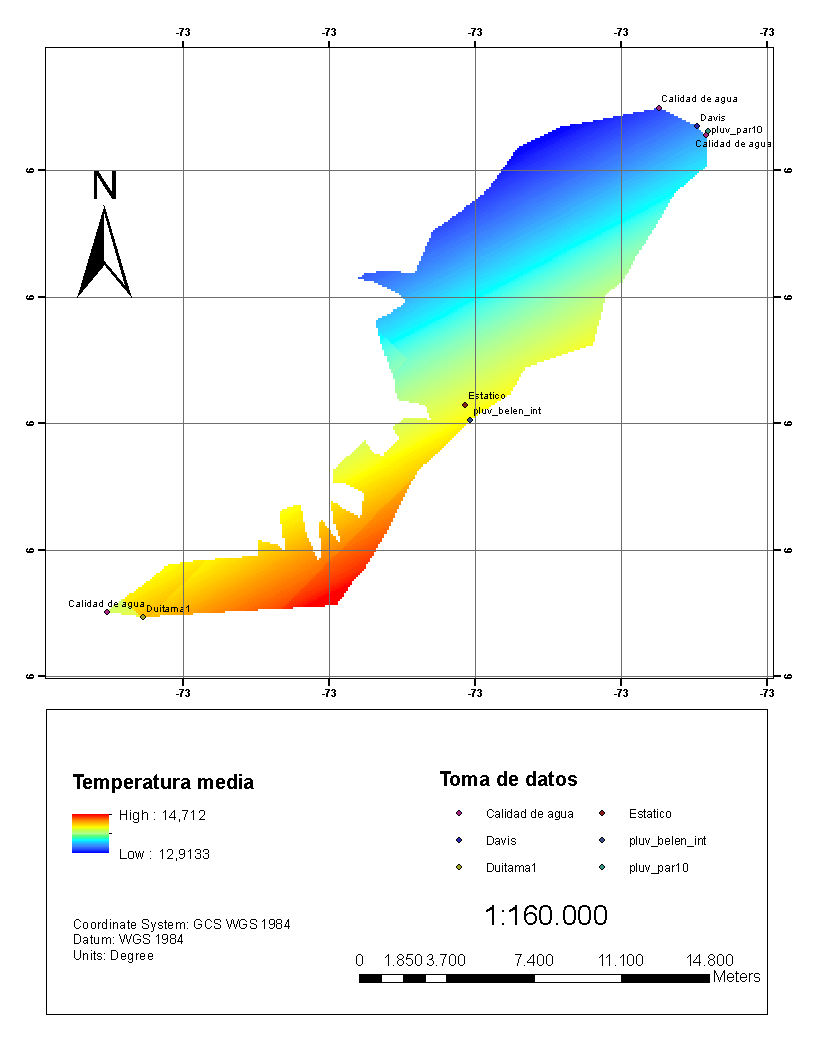
\includegraphics{paramo3.png}
\caption{Modelo de temperatura}
\end{figure}

\hypertarget{conclusiones}{%
\section{Conclusiones}\label{conclusiones}}

El clima en el páramo de La Rusia presenta la variabilidad esperada con
su temperatura máxima de \(19.5^{\circ}C\) a medio día y una mínima de
\(1.6^{\circ}C\) en la madrugada, una humedad relativa constantemente
alta en excepción del tiempo donde se tiene la temperatura más alta
haciendo de este un páramo muy húmedo, que si se tiene una buena
regeneración del ecosistema con unos suelos ricos en porosidad y óptimos
en infiltración, ayudado de la vegetación, puede ser muy importante para
la captura de agua y alimentación de los acuíferos subterráneos y ríos,
proporcionando así una buena oferta hídrica. Por lo que se hace
necesario estudios más detallados para la conservación de estos
ecosistemas sobre todo en un país como Colombia que tiene la mitad de
páramos del mundo en el cual cae la responsabilidad en sus ciudadanos
para un manejo óptimo y sostenible.

\bibliography{mybibfile}

\end{document}


